%%%%%%%%%%%%%%%%%%%%%%%%%%%%%%%%%%%%%%%%%%%%%%%%%%%%%%%%%%%%%%%%%%%%%%%%%%% 
% 
% Generic template for TFC/TFM/TFG/Tesis
% 
% By:
% + Javier Macías-Guarasa. 
% Departamento de Electrónica
% Universidad de Alcalá
% + Roberto Barra-Chicote. 
% Departamento de Ingeniería Electrónica
% Universidad Politécnica de Madrid   
% 
% Based on original sources by Roberto Barra, Manuel Ocaña, Jesús Nuevo,
% Pedro Revenga, Fernando Herránz and Noelia Hernández. Thanks a lot to
% all of them, and to the many anonymous contributors found (thanks to
% google) that provided help in setting all this up.
% 
% See also the additionalContributors.txt file to check the name of
% additional contributors to this work.
% 
% If you think you can add pieces of relevant/useful examples,
% improvements, please contact us at (macias@depeca.uah.es)
% 
% You can freely use this template and please contribute with
% comments or suggestions!!!
% 
%%%%%%%%%%%%%%%%%%%%%%%%%%%%%%%%%%%%%%%%%%%%%%%%%%%%%%%%%%%%%%%%%%%%%%%%%%% 

\chapter{Experimental Results and Applications}
\label{cha:experimental_results_and_applications}

\begin{FraseCelebre}
	\begin{Frase}
		La fuerza de tus convicciones \\
		determina tu éxito, \\
		no el número de tus seguidores.
	\end{Frase}
	\begin{Fuente}
		Reamus Lupin \\
		Harry Potter y Las Reliquias de la Muerte, Parte 2
	\end{Fuente}
\end{FraseCelebre}

\section{Introduction}
\label{sec:5_introduction}

In this section we will detail the experiments carried out to assess the performance both in terms of accuracy and computational resources (time, \acp{FLOP}, parameters) for real-time \ac{MP} applications in the field of \ac{AD}.

\section{SmartMOT results}
\label{sec:5_mot_and_euroncap}

\subsection{Multi-Object Tracking results}
\label{sec:5_mot_results}

In order to evaluate our proposed \ac{MOT} system pipeline, we carry out the evaluation in the KITTI \ac{MOT} benchmark based on the method proposed by \cite{weng20203d}. The KITTI MOT benchmark is composed of 29 testing and 21 training video sequences, where each sequence is provided with the corresponding RGB images (left and right camera of the stereo pair), LiDAR point cloud and the corresponding calibration file. Since KITTI does not provide any annotation (i.e., the groundtruth) for the testing split, we decided to evaluate our system in the training/validation split, which contains 636 and 30,601 annotated trajectories and objects respectively. Moreover, although KITTI distinguish among eight different classes for the object type, our work focus on the car subset, since it is the class that contains the most number of instances over the whole benchmark.

Mainstream metrics applied to MOT systems are extracted from CLEAR MOT metrics \cite{bernardin2008evaluating}, such as MOTA (Multi-Object Tracking Accuracy), MOTP (Multi-Object Tracking Precision), ML/MT (Number of Mostly Lost/Tracked trajectories), IDS (Number of identity swutches), FRAG (Number of fragmentations generated by false negatives) and FN/FP (Number of false negatives/positives). These metrics provide a comprehensive assessment of tracking performance by considering aspects such as accuracy, precision, and overall performance:

\paragraph{MOTA (Multi-Object Tracking Accuracy)}
	
The MOTA metric is commonly used to evaluate the performance of multi-object tracking algorithms. It measures the overall tracking accuracy by considering the false positives (FP), false negatives (FN), and identity switches (IDS) in the tracking results. The formula for calculating MOTA is given as:

\begin{equation}
MOTA = 1 - \frac{{\text{{FN}} + \text{{FP}} + \text{{IDS}}}}{{\text{{GT}}}}
\end{equation}

where:
\begin{itemize}
	\item FN (False Negatives) represents the number of ground truth objects that were not correctly detected by the tracking algorithm.
	\item FP (False Positives) represents the number of false detections made by the tracking algorithm.
	\item IDS (Identity Switches) represents the number of times the algorithm incorrectly switches the identity of a tracked object.
	\item GT (Ground Truth) represents the total number of ground truth objects in the video sequence.
\end{itemize}

A higher MOTA value indicates better tracking accuracy, with a perfect tracking result yielding MOTA = 1.

\paragraph{MOTP (Multi-Object Tracking Precision)}

The MOTP metric is used to assess the localization accuracy of a multi-object tracking algorithm. It measures the average precision of the tracked object positions by considering the distance between the predicted locations and their corresponding ground truth locations. The formula for calculating MOTP is given as:

\[
MOTP = \frac{{\sum_{{i=1}}^{{N}} d_i}}{{N}}
\]

where:
\begin{itemize}
	\item \(N\) represents the total number of matched object pairs between the predicted and ground truth locations.
	\item \(d_i\) represents the Euclidean distance between the predicted location and the ground truth location for the \(i\)-th matched object pair.
\end{itemize}

The MOTP metric ranges between 0 and 1, with a higher value indicating better localization accuracy. A perfect tracking result with exact object positions would yield MOTP = 1.

\paragraph{Integral metrics: AMOTA and AMOTP}

Nevertheless, these metrics analyze the DAMOT system performance at a given threshold, not taking into account the confidence provided by the object detector and possibly misunderstanding the capability of the method. That means they do not take into account the full spectrum of precision and accuracy over different thresholds. Moreover, these traditional metrics evaluate the performance of the MOT system on the image plane (by projecting the detected 3D bounding box onto the image plane), which does not demonstrate the full strength of 3D DATMO. In that sense, AB3DMOT \cite{weng20203d} recently presented a 3D extension of the KITTI 2D MOT evaluation, known as KITTI-3DMOT, which focuses on the dimensions, orientation and centroid position of the 3D bounding box instead of the projection onto the image plane to evaluate the performance of the MOT system. Moreover, two new integral MOT metrics are introduced in order to solve the problem of evaluating the MOTA and MOTP of the system across all thresholds, known as AMOTA and AMOTP (Average MOTA and MOTP), as shown in Equation \ref{5_amota}:

\begin{equation}
	\label{eq:5_amota}
	AMOTA = \frac{1}{L}\sum_{\{\frac{1}{L},\frac{2}{L},...,1\}}(1-\frac{FP+FN+IDS}{num_{gt}})
\end{equation}

Where $L$ is the number of different recall values. Note that IDS, FP and FN are modified according to the results of each threshold value. Likewise, AMOTP can be estimated by integrating MOTP across all recall values.

\subsection{MOT ablation study}
\label{subsec:5_mot_ablation}

\subsection{MOT leaderboard results}
\label{subsec:5_mot_}

\subsection{EuroNCAP-based validation}
\label{sec:5_euroncap}

A considerable amount of research works and studies, related to pedestrian detection and collision avoidance behavior are present in the literature, where the main objective is to validate the perception and control modules. Nevertheless, as state before our goal to demonstrate how incorporating HD map information helps the whole AD stack to anticipate faster the behaviour of the traffic participants in the corresponding traffic scenarios. Then, common metrics for all frameworks must be used to evaluate the whole architecture, where all modules are integrated. Regarding this, New Car Assessment Programs (NCAPs) protocols are introduced, evaluating the safety of vehicles for different traffic situations and Advanced Driver Assistance Systems, such as Child Occupant Protection (COP), Speed Assist Systems (SAS) or Autonomous Emergency Braking (AEB). Euro-NCAP \cite{article_EuroNCAP_2} is introduced in 1997, representing the widely most adopted performance assessment within the scope of the collaboration of European Union countries. China New Car Assessment Program (C-NCAP) \cite{article_CNCAP} is presented (2006) as a research and development benchmark for vehicle manufacturers in Asia, being most of its protocols based on Euro-NCAP. National Highway Transportation Safety Administration (NHTSA), funded in 1970 as an agency of the Department of Transportation of United States, published \cite{article_NHTSA} its guidance documents and regulations on vehicles equipped with ADAS. As observed, these programmes do not present specific protocols in order to evaluate AD stacks, presenting noticeable differences, such as different scenarios, parameters and evaluation metrics. Then, we adop the validation method proposed by \cite{gutierrez2021validation}, which proposes to generalize the VRU v.10.0.3 protocol \cite{web_VRU_assessment_protocol}, representing a baseline to compare the performance of different pipelines for the particular situation (both in simulation and real-world) of an Unexpected Vulnerable Road User (VRU) jumping into the road during the navigation, where an Autonomous Emergency Braking (AEB) behaviour must be executed. 

\subsubsection{Implementation details of the EuroNCAP scenario}
\label{sec:5_euroncap_implementation_details}

Figure \ref{fig:5_cpna_scenario} illustrates this traffic situation, in which the VRU (a pedestrian in this particular case) starts in the closest sidewalk to the vehicle in a perpendicular position to the vehicle orientation. Once the vehicle starts the navigation and the L2 distance between the ego-vehicle centroid and the VRU centroid is lower than a certain threshold \textit{d}, the VRU starts its path to unexpectedly cross the road in such a way the ego-vehicle must detect, track and forecast its future trajectory in order to avoid the collision or at least reduce the impact velocity as much as possible. Then, the protocol consists on reproducing the CPNA crash avoidance scenario, with a fixed VRU velocity (\(v_p\)) of 5 km/h and a variable ego-vehicle velocity that ranges from 10 km/h to 60 km/h. It is important to note that the threshold \textit{d} is not fixed, but it is ego-vehicle velocity dependent, that is, the pedestrian must start walking in such a way the impact point (\(P_I\)) (Figure \ref{fig:5_cpna_scenario}) is in the center of the lane for each particular velocity. 

\begin{figure}[h]
	\centering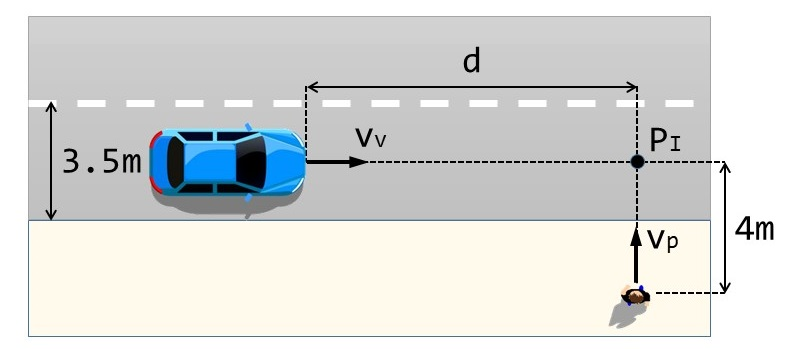
\includegraphics[width=0.4\textwidth]{5_CPNA_scenario.jpg}
	\caption{Car to Pedestrian Nearside Adult (CPNA) scenario}	
	\label{fig:5_cpna_scenario}
\end{figure}

Regarding the evaluation metrics, a score for each test is calculated based on the velocity reduction of the vehicle, as following:

\begin{itemize}
	\item For a vehicle velocity \(v_v\) less than or equal to 40km/h:
	\begin{itemize}
		\item If the vehicle stops without collision, the highest score is achieved:
		\begin{equation}
			score_{test} = score_{max}
			\label{eq1}
		\end{equation}
		
		\item Otherwise, if the vehicle collides, its score is defined as follows:
		\begin{equation}
			score_{test} = \frac{v_{test}-v_{impact}}{v_{test}} \cdot score_{max}
			\label{eq2}
		\end{equation}
	\end{itemize}
	\item For \(v_v\) higher than 40km/h:
	\begin{itemize}
		\item If the vehicle is able to reduce its speed in at least 20 km/h, the highest score is achieve:
		\begin{equation}
			v_{impact} \leq v_{test} - 20 \to score_{test} = score_{max}
			\label{eq3}
		\end{equation}
		\item Otherwise, if the vehicle collides at a velocity greater than the velocity under test less a threshold of 20 km/h, no score is achieve:
		\begin{equation}
			v_{impact} > v_{test} - 20 \to score_{test} = 0
			\label{eq4}
		\end{equation}
	\end{itemize}
\end{itemize}

Finally, the final score of a particular pipeline is given by the arithmetic mean of the results obtained in each CPNA crash avoidance test for different weather conditions. For further details about the validation protocol, we refer the reader to \cite{gutierrez2021validation}.

\subsubsection{Experimental results EuroNCAP scenario}
\label{sec:5_euroncap_experimental_results}

In this section we obtain some interesting both qualitative and quantitative results, evaluating our AD stack \cite{gomez2021train} in the CPNA crash avoidance scenario using two different perception layer strategies. On the one hand, we implement the perception module stated by \cite{gomez2020real} which tracks all objects in the environment regardless their topological information and considers a naive velocity dependent rectangular monitored area in front of the vehicle to determine the distance to the nearest object in the route as well as to predict the collision. On the other hand, we use SmartMOT to track and predict the future trajectories of only the most relevant obstacles around the vehicle, that is, those in which the human in manual driver should pay attention throughout the route, such as VRUs close to the road, vehicles in intersections and lanes where the lane change maneuver is allowed, etc. Qualitative results may be found in the following play list \href{https://cutt.ly/uk9ziaq}{SmartMOT} \footnote{SmartMOT: https://cutt.ly/uk9ziaq}, where the SmartMOT performance is illustrated. 

Regarding urban environment complexity, in order to validate a whole AD architecture the system must be tested in countless environments and scenarios, which would escalate the cost and development time exponentially with a physical approach. Considering this, the use of photo-realistic simulation (virtual development and validation testing) and an appropriate design of the driving scenarios are the current keys to build safe and robust AV. In our work we propose the use of CARLA (CAR Learning to Act) \cite{carla} as the best open-source simulator to reach our goals, taking even more importance when analyzing the behaviours the vehicle can face in these complex traffic scenarios. One of the best advantages of CARLA is the possibility to create ad-hoc urban layouts, useful to validate the navigation architecture in challenging driving scenarios. This code can be downloaded from the ScenarioRunner repository, associated to the CARLA GitHub. The ScenarioRunner is a module that allows the user to define and execute traffic scenarios for the CARLA simulator. In the present case, we define several scenarios according to the CPNA crash avoidance traffic situation, modifying the velocity of the ego-vehicle and the presence of other traffic participants. All test were carried out in a PC desktop (Intel Core i7-9700k, 32GB RAM with CUDA-based NVIDIA GeForce RTX 2080 Ti 11GB VRAM), using the version 0.9.10.1 version of CARLA as well as the corresponding ROS Bridge, responsible of communicating the CARLA environment with our ROS-based architecture, and ScenarioRunner modules. In particular, we make use of the OpenScenario standard, supported by ScenarioRunner, where both the VRU and ego-vehicle features can be modified to accomplish the Euro-NCAP requirements. Due to size constraint of this paper, we do not validate the performance of our architecture for different weather conditions but only in daytime conditions. 

In order to appreciate the behaviour of the vehicle during navigation, we incorporate a very illustrative temporal diagram (Figure \ref{fig:5_unexpected_vru}), representing a powerful manner to qualitatively validate how the architecture behaves in an end-to-end manner, since we can observe how the car behaves considering the different actions and events \cite{gomez2021train} provided by the executive layer, which is actually the output of the whole architecture before sending commands to the motor. As observed, the ego-vehicle starts far away from the adversary and starts its navigation. At second 22 a pedestrian that is in the sidewalk is detected, so tracking-by-detection and subsequent motion prediction must be carried as fast as possible to avoid collision, since the scenario is designed in such a way that the pedestrian must start walking in such a way the impact point (\(P_I\)) (Fig. \ref{cpna_scenario}) is in the center of the lane for each particular velocity. After that, our prediction module intersects the ego-vehicle forecasted trajectory and the pedestrian forecasted trajectory. If the Intersection over Union (IoU) is greater than a threshold (in this case, 0.01), a \textit{predictedcollision} flag is activated and the low-level (reactive) control, which always runs in the background of the decision-making layer, performs an emergency break until the car is stopped in front of the obstacle. Navigation is resumed once the obstacle leaves the driving lane. Table \ref{table:CPNA_results} compares the performance of the architecture by implementing \cite{gomez2020real} and a rectangular monitorized lane to retrieve the nearest object in route and predict collision against our proposal, where it can be appreciated that for velocities greater than 40 km/h, using HD map semantic and geometric information gives the car a valuable reaction time to anticipate the VRU behaviour and avoid the collision, achieving the highest score. 

\begin{table}[]
	\centering
	\caption{Comparison of our two different perception strategies in the Car to Pedestrian Nearside Adult (CPNA) scenario. We bold the best score in \textbf{black}}
	\label{table:CPNA_results}
	\begin{tabular}{c | c | c  c | c  c  } 
		\hline 
		\multicolumn{6}{c}{\textbf{CPNA}}\\
		\hline \hline
		\multirow{2}{*}{\textbf{\(v_{test}\)}} & \multirow{2}{*}{\textbf{\(score_{max}\)}} & \multicolumn{2}{c}{\textbf{Rectangular area + \cite{gomez2020real}}} & \multicolumn{2}{c}{\textbf{SmartMOT}} \\ 
		& & \(v_{impact}\) & \(score\) & \(v_{impact}\) & \(score\) \\
		\hline
		10 km/h & 1.00 & 0.0 km/h & 1.00 & 0.0 km/h & 1.00 \\
		20 km/h & 1.00 & 0.0 km/h & 1.00 & 0.0 km/h & 1.00 \\
		30 km/h & 2.00 & 0.0 km/h & 2.00 & 0.0 km/h & 2.00 \\
		40 km/h & 3.00 & 0.0 km/h & 3.00 & 0.0 km/h & 3.00 \\
		50 km/h & 2.00 & 23.82 km/h & 2.00 & 0.0 km/h & 2.00 \\
		60 km/h & 1.00 & 44.23 km/h & 0.00 & 0.0 km/h & 1.00  \\
		\hline \hline
		\textbf{Total} & 10.00 &  & 9.00 & & \textbf{10.0} \\
		\hline
	\end{tabular}
\end{table}

Figure \ref{graphics} shows different analysis of the CPNA crash avoidance scenario with variable ego-vehicle and the incorporation of other traffic participants in the scenario (\ref{subfig:3} \ref{subfig:4}). \(T_0\) corresponds with the moment the vehicle either stops or collides, and crosses \textbf{x} represent the moment in which the system sends a predicted collision signal to the executive layer, so it is coherent that crosses in tests where the ego-vehicle collides with the VRU are shifted to the right (prediction collision signal was given in time). Left column tracks all objects around the vehicle and adopts a geometric monitorized area to estimate the nearest distance and predicted collision, whilst right column uses HD map information to help in the Multi-Object Tracking and motion prediction tasks, monitorizing only the most relevant traffic participants around the vehicle that is, SmartMOT. Using HD map information is able to avoid collision until a ego-vehicle velocity of 80 km/h, where SmartMOT is not able to send a signal of predicted collision (output of the system, as shown in Fig. \ref{system_pipeline}) in time, colliding at a velocity of 39.78 km/h. Nevertheless, this velocity at the moment of collision is even lower that the impact velocity (44.23 km/h) when testing the system under 60 km/h condition not using HD map in the MOT stage, illustrating how incorporating additional semantic and geometric map information helps the vehicle to react faster or at least mitigate the effect of collision. Moreover, we simulate both perception strategies using the most common velocities in urban scenarios, which range from 30 to 50 km/h, including \ref{subfig:3} \ref{subfig:4} static adversaries (in particular, vehicles and pedestrians) which do not actually in the traffic scenario to fulfill the particular requirements stated by \cite{felipe} protocol. As expected, tracking all objects around the ego-vehicle and using the rectangular monitorized area suffers when the number of traffic participants is increased around the ego-vehicle, whilst SmartMOT holds this exponential increase by analyzing the objects and their corresponding role as relevant obstacles considering the information provided by the HD map, avoiding the collision in all situations.

\begin{figure}[ht]
	\centering
	\begin{subfigure}{0.45\textwidth}
		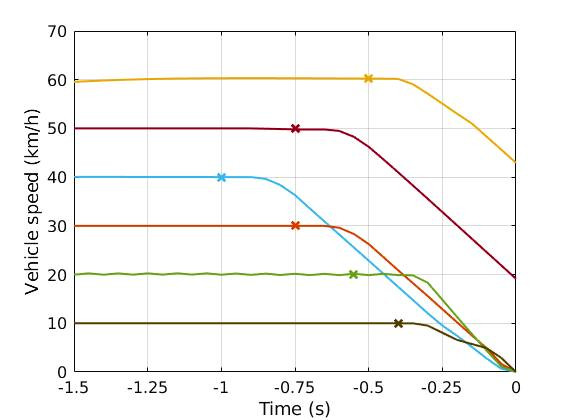
\includegraphics[width=\textwidth]{5_euroncap_without_adversaries_geometric.jpg}
		\caption{Rectangular monitored area without adversaries}
		\label{fig:5_euroncap_graphics_a}
	\end{subfigure}
	\hfill
	\begin{subfigure}{0.45\textwidth}
		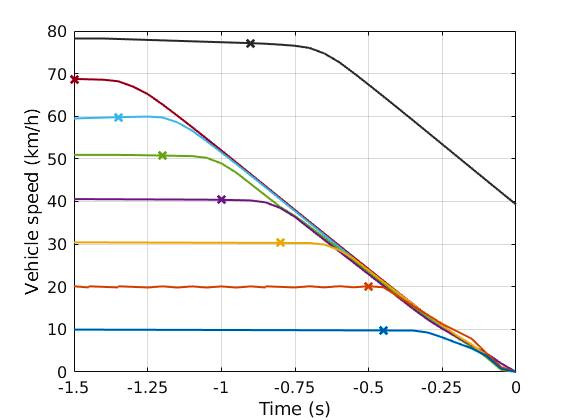
\includegraphics[width=\textwidth]{5_euroncap_without_adversaries_hdmap.jpg}
		\caption{SmartMOT area without adversaries}
		\label{fig:5_euroncap_graphics_b}
	\end{subfigure}
	\hfill
	\begin{subfigure}{0.45\textwidth}
		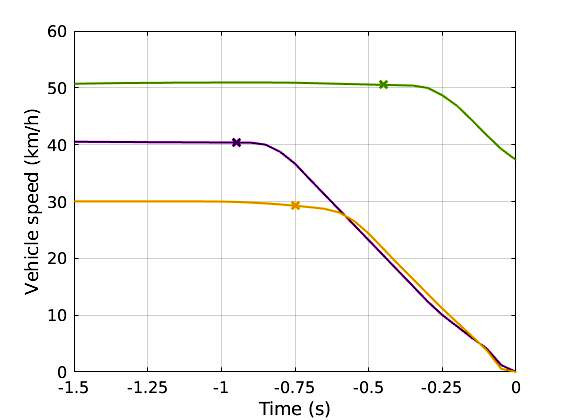
\includegraphics[width=\textwidth]{5_euroncap_with_adversaries_geometric.jpg}
		\caption{Rectangular monitored area with adversaries}
		\label{fig:5_euroncap_graphics_c}
	\end{subfigure}
	\hfill
	\begin{subfigure}{0.45\textwidth}
		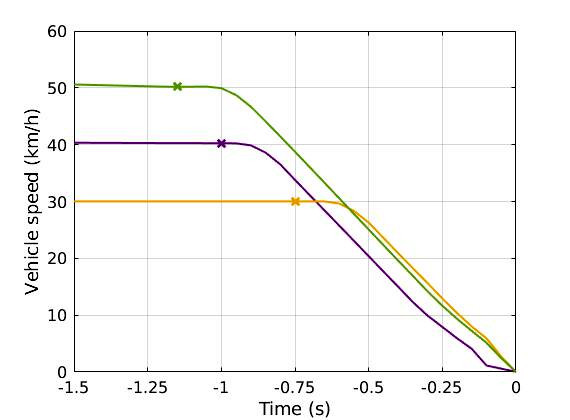
\includegraphics[width=\textwidth]{5_euroncap_with_adversaries_hdmap.jpg}
		\caption{SmartMOT area with adversaries}
		\label{fig:5_euroncap_graphics_d}
	\end{subfigure}

	\caption[Analysis of the Car to Pedestrian Nearside Adult (CPNA) crash avoidance scenario with variable ego-vehicle velocity]{Analysis of the Car to Pedestrian Nearside Adult (CPNA) crash avoidance scenario with variable ego-vehicle velocity. Left column (Figures \ref{fig:5_euroncap_graphics_a} and \ref{fig:5_euroncap_graphics_c}) adopts a rectangular monitorized area to estimate the nearest distance and predicted collision, Right column (Figures \ref{fig:5_euroncap_graphics_b} and \ref{fig:5_euroncap_graphics_d}) uses HD map information for this purpose. On the other hand, first row shows the scenario without additional traffic participants, second row analyzes the crash avoidance scenario including additional traffic participants to the road, monitorized sidewalk area and non-relevant sidewalk area. Crosses in the lines represent the moment in which the system sends a predicted collision signal to the executive layer}
	\label{fig:5_cpna_results}
\end{figure}

\begin{figure*}[h]
	\centering
	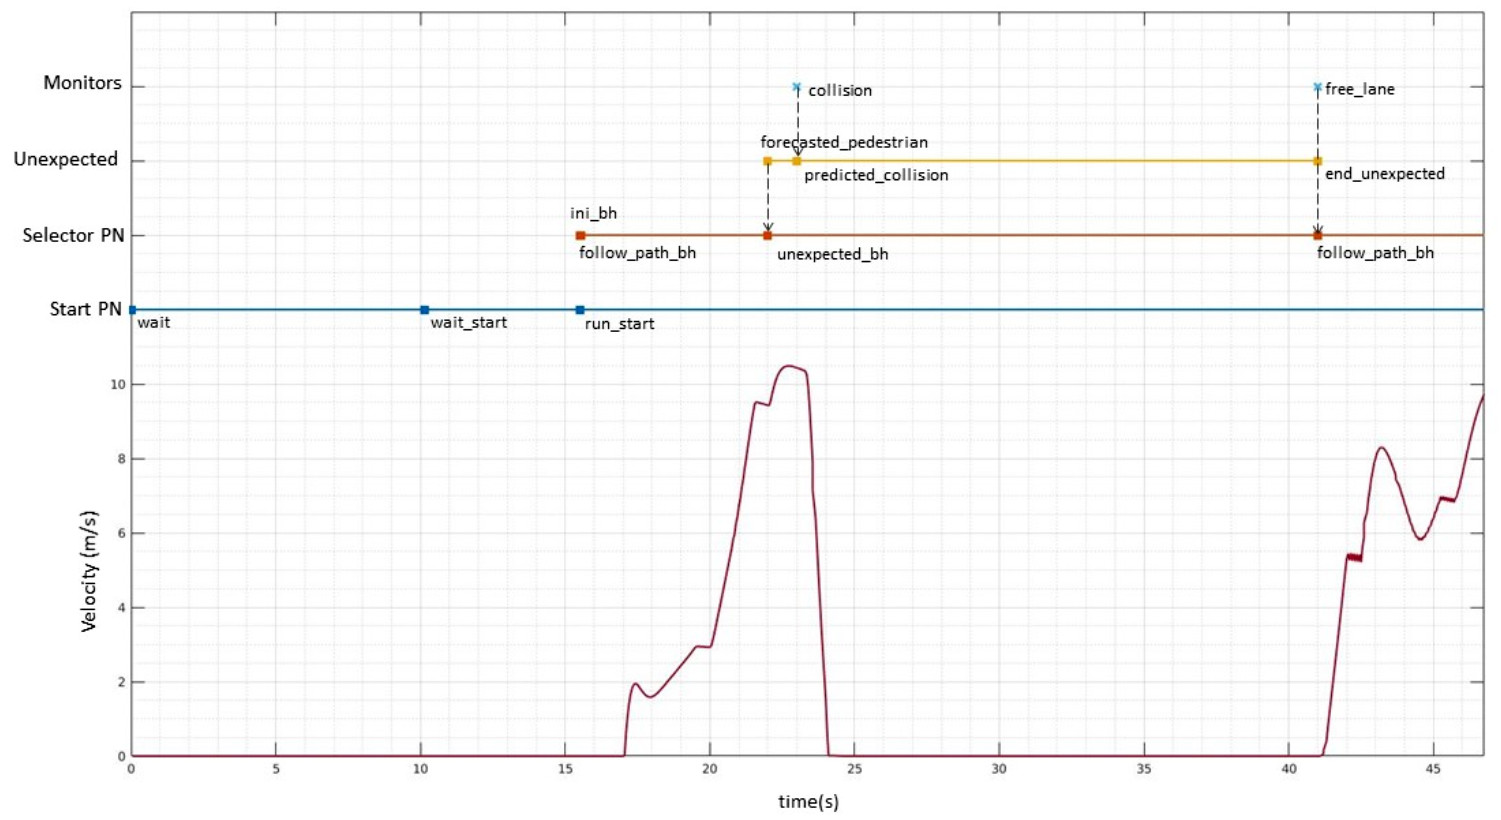
\includegraphics[width=0.8\textwidth]{5_Unexpected_Pedestrian_Temporal_Graph.jpg}
	\caption[Unexpected Vulnerable Road User (VRU) temporal diagram]{Unexpected Vulnerable Road User (VRU) temporal diagram. At the top, the events produced by our monitors and map manager modules. In the middle, the selector, and start (background) PNs of our decision-making layer. At the bottom, the velocity of the car throughout the navigation}
	\label{fig:5_unexpected_vru}
\end{figure*}

\section{Motion Prediction Datasets}
\label{sec:5_motion_prediction_datasets}

For motion forecasting, the progress has been just as significant. A transition to attention-based methods \cite{Mercat19arxiv_MultiheadAttentionForecasting, Mercat20icra_MultiheadAttentionForecasting} has led to a variety of new vector-based representations for map and trajectory data \cite{Gao20cvpr_VectorNet,Liang20eccv_LaneGCN}. New datasets have also paved the way for new algorithms, with nuScenes \cite{Caesar20cvpr_NuScenes}, Lyft L5 \cite{Houston20arxiv_LyftL5}, and the Waymo Open Motion Dataset \cite{Ettinger21arxiv_WaymoOpenMotion} all releasing lane graphs after they proved to be essential in Argoverse 1~\cite{Chang19cvpr_Argoverse}. Lyft  also introduced traffic/speed control data, while Waymo added crosswalk polygons, lane boundaries (with marking type), speed limits, and stop signs to the map. More recently, Yandex has released the Shifts \cite{Malinin21arxiv_ShiftsYandex} dataset, which is the largest (by scenario hours) collection of forecasting data available to date. Together, these datasets have enabled exploration of multi-actor, long-range motion forecasting leveraging both static and dynamic maps.

Following upon the success of Argoverse 1.1, we position AV2 as a large-scale repository of high-quality motion forecasting scenarios - with guarantees on data frequency (exactly 10 Hz) and diversity (>2000 km of unique roadways covered across 6 cities). This is in contrast to nuScenes (reports data at just 2 Hz) and Lyft (collected on a single 10 km segment of road), but is complementary to Waymo Open Motion Dataset (employs a similar approach for scenario mining and data configuration). Complementary datasets are essential for these safety critical problems as they provide opportunities to evaluate generalization and explore transfer learning. To improve ease of use, we have also designed AV2 to be widely accessible both in terms of data size and format --- a detailed comparison vs. other recent forecasting datasets is provided in Table \ref{forecasting-comparison}.

As stated throughout this thesis, Motion Prediction addresses the problem of predicting future states (or occupancy maps) for dynamic actors within a local environment. Some examples of relevant actors for autonomous driving include: vehicles (both parked and moving), pedestrians, cyclists, scooters, and pets. Predicted futures generated by a forecasting system are consumed as the primary inputs in motion planning, which conditions trajectory selection on such forecasts. Generating these forecasts presents a complex, multi-modal problem involving many diverse, partially-observed, and socially interacting agents. However, by taking advantage of the ability to ``self-label'' data using observed ground truth futures, motion forecasting becomes an ideal domain for application of machine learning. 

\begin{table}[t]
	\caption{Comparison between the Argoverse 2 Motion Forecasting dataset and other recent motion forecasting datasets. Hyphens "-" indicate that attributes are either not applicable, or not available. We define ``mined for interestingness'' to be true if interesting scenarios/actors are mined \textit{after data collection}, instead of taking all/random samples. $\dagger$ Public leaderboard counts as retrieved on Aug. 27, 2021.}
	\label{forecasting-comparison}
	\centering
	\begin{adjustbox}{max width=\columnwidth}
		\begingroup
		\renewcommand{\arraystretch}{1.25} %
		\begin{tabular}{rccccccc}
			\toprule
			& \textsc{Argoverse 1}~\cite{chang2019argoverse} & \textsc{Interaction}~\cite{zhan2019interaction} & \textsc{Lyft}~\cite{john2020one} & \textsc{Waymo}~\cite{ettinger2021large} & \textsc{NuScenes}~\cite{caesar2020nuscenes} & \textsc{Yandex}~\cite{malinin2021shifts} & \textsc{Argoverse 2}~\cite{malinin2021shifts} \\
			\midrule
			\textsc{\# Scenarios} & 324k & - & 170k & 104k & 41k & 600k & 250k \\
			\textsc{\# Unique Tracks} & 11.7M  & 40k & 53.4M & 7.6M & - & 17.4M & 13.9M  \\
			\textsc{Average Track Length} & 2.48 s & 19.8 s & 1.8 s & 7.04 s & - & - & 5.16 s  \\
			\textsc{Total Time} & 320 h & 16.5 h & 1118 h & 574 h & 5.5 h & 1667 h & 763 h \\
			\textsc{Scenario Duration} & 5 s & - & 25 s & 9.1 s & 8 s & 10 s & 11 s \\
			\textsc{Test Forecast Horizon} & 3 s & 3 s & 5 s & 8 s & 6 s & 5 s & 6 s \\
			\textsc{Sampling Rate} & 10 Hz & 10 Hz & 10 Hz & 10 Hz & 2 Hz & 5 Hz & 10 Hz \\
			\textsc{\# Cities} & 2 & 6 & 1 & 6 & 2 & 6 & 6  \\
			\textsc{Unique Roadways} & 290 km & 2 km & 10 km & 1750 km & - & - & 2220 km \\
			\textsc{Avg. \# tracks per scenario} & 50 & - & 79 & - & 75 & 29 & 73\\
			\textsc{\# Evaluated object categories} & 1 & 1 & 3 & 3 & 1 & 2 & 5 \\
			\textsc{Multi-agent evaluation} & $\times$ & \checkmark & \checkmark & \checkmark & $\times$ & \checkmark &\checkmark \\
			\textsc{Mined for Interestingness} & \checkmark & $\times$ & - & \checkmark & $\times$ & $\times$ & \checkmark \\
			\textsc{Vector Map} & \checkmark & $\times$ & $\times$ & \checkmark & \checkmark & $\times$ &\checkmark \\
			\textsc{Download Size} & 4.8 GB  & -  & 22 GB  & 1.4 TB  & 48 GB & 120 GB & 58 GB \\
			\textsc{\# Public Leaderboard Entries}$^\dagger$ & 194  & -  & 935  & 23 & 18 & 3 & - \\
			\bottomrule
		\end{tabular}
		\endgroup
	\end{adjustbox}
\end{table}

Comparing different motion prediction datasets in the field of autonomous driving can help understand their characteristics, applications, and limitations. Here is an extensive comparison among the various motion prediction datasets you mentioned: Argoverse 1, Interaction, Lyft, Waymo, NuScenes, Yandex, and Argoverse 2.

Argoverse 1:
Dataset Description: Argoverse 1 focuses on motion forecasting for autonomous vehicles, containing high-definition maps, detailed vehicle sensor data, and 3D object detection annotations.
Data Size: Contains 5,000 scenes with 324,557 labeled objects.
Features: Provides sensor data from lidar, camera, and radar, along with accurate ground truth trajectories for objects.
Applications: Useful for predicting the future motions of surrounding objects to enable safe and efficient autonomous driving.
Limitations: Limited to urban environments, does not include interaction data with human-driven vehicles.

Interaction:
Dataset Description: Interaction dataset emphasizes capturing interactions between different traffic participants for motion prediction.
Data Size: Contains 9,933 scenes with over 4 million annotated object instances.
Features: Provides high-resolution lidar data, radar data, and object annotations.
Applications: Suitable for modeling complex interaction scenarios and studying multi-agent motion prediction.
Limitations: Limited geographic coverage, predominantly focused on urban environments.

Lyft:
Dataset Description: Lyft dataset focuses on autonomous vehicle perception and prediction, providing sensor data, object annotations, and human-driven trajectories.
Data Size: Contains more than 55,000 human-driven vehicle trajectories.
Features: Offers high-resolution lidar data, camera images, and HD maps, along with accurate object annotations.
Applications: Used for perception and prediction tasks, including motion forecasting and behavior prediction.
Limitations: Limited coverage of scenarios, restricted to a few cities.

Waymo:
Dataset Description: Waymo dataset comprises sensor data from a diverse range of scenarios, recorded by Waymo self-driving cars.
Data Size: Consists of approximately 1,000 driving segments with various road and weather conditions.
Features: Provides high-resolution lidar data, camera images, radar data, and HD maps, along with object annotations and behavior labels.
Applications: Suitable for perception, prediction, and planning tasks in autonomous driving systems.
Limitations: Dataset access is limited, and the exact data size and coverage are not publicly disclosed.

NuScenes:
Dataset Description: NuScenes dataset focuses on capturing diverse urban driving scenarios and provides sensor data, object annotations, and HD maps.
Data Size: Contains over 1,400 scenes with more than 1.4 million object annotations.
Features: Offers lidar data, camera images, radar data, HD maps, and object annotations.
Applications: Used for perception, prediction, and planning tasks, including motion forecasting and behavior modeling.
Limitations: Limited to urban environments and specific geographic locations.

Yandex:
Dataset Description: Yandex dataset includes sensor data recorded by Yandex self-driving cars in various real-world driving scenarios.
Data Size: Exact data size is not publicly disclosed.
Features: Provides lidar data, camera images, and object annotations.
Applications: Suitable for perception, prediction, and planning tasks in autonomous driving systems.
Limitations: Dataset access is limited, and specific details regarding data size and coverage are not publicly available.

Argoverse 2:
Dataset Description: Argoverse 2 dataset is an extension of Argoverse 1, focusing on 3D object detection, tracking, and motion forecasting for autonomous driving.
Data Size: Exact data size is not publicly disclosed.
Features: Provides lidar data, camera images, radar data, HD maps, and accurate object annotations.
Applications: Useful for perception, prediction, and planning tasks in autonomous driving systems.
Limitations: Specific details regarding data size and coverage are not publicly available.

Overall, these datasets have common goals of enabling motion prediction and improving the safety and efficiency of autonomous driving systems. However, their coverage, data size, features, and limitations vary, which makes it important to consider the specific requirements and use cases when choosing a dataset for research or development purposes.

\subsection{Argoverse 1 Motion Forecasting dataset}
\label{subsec:5_argoverse_1}

The Argoverse 1 Motion Forecasting dataset is a widely used dataset in the field of autonomous driving for studying and developing algorithms related to motion prediction. Here is an extensive review of the dataset:

Dataset Description:
The Argoverse 1 dataset focuses on motion forecasting for autonomous vehicles.
It includes high-definition maps, detailed sensor data, and 3D object detection annotations.
The dataset provides sensor data from lidar, camera, and radar sensors.
The object annotations include accurate ground truth trajectories for objects in the scene.
It contains a diverse set of urban driving scenarios, enabling researchers to study various complex situations.

Data Size:
The dataset comprises a significant amount of data, offering ample resources for training and evaluation.
It contains a total of 5,000 scenes with 324,557 labeled objects.
The scenes are captured from multiple cities, ensuring geographic diversity.

Features:
The dataset provides rich sensor data, including lidar point clouds, camera images, and radar sweeps.
Lidar data offers detailed 3D information about the surrounding environment, which is crucial for accurate motion prediction.
Camera images provide visual context and object appearance information.
Radar data helps capture the velocity and movement of objects.
High-definition maps are available, aiding in localization and understanding the road structure.

Applications:
The Argoverse 1 dataset is primarily designed for motion forecasting and prediction tasks in autonomous driving.
It is suitable for developing algorithms that predict the future motions of surrounding objects to enable safe and efficient autonomous driving.
The dataset can be utilized for research, benchmarking, and development of motion prediction models and algorithms.

Evaluation Metrics:
The dataset provides ground truth trajectories for objects, allowing for quantitative evaluation of motion prediction algorithms.
Common evaluation metrics, such as mean average displacement error (ADE) and final displacement error (FDE), can be used to measure the accuracy of predicted trajectories compared to ground truth.

Limitations:
The dataset is focused on urban driving scenarios, limiting its applicability to specific environments.
It does not include explicit interaction data with human-driven vehicles, which is an important aspect of motion prediction.
While the dataset provides a substantial amount of labeled data, it may still have limitations in capturing the full diversity of real-world driving scenarios.

In summary, the Argoverse 1 Motion Forecasting dataset is a valuable resource for researchers and developers working on motion prediction in the field of autonomous driving. With its diverse urban driving scenarios, rich sensor data, and ground truth annotations, the dataset enables the development and evaluation of robust motion forecasting algorithms.

 \begin{table}[!ht]
	\centering
	\caption{\textbf{Error comparison} (in terms of $\mathcal{L}_2$~distance) between the target agent ground-truth end-point and proposed centerlines end-points with different preprocessing methods in the validation split (39,472 samples). CTRV and CTRA stand for \textit{Constant Turn Rate Velocity} and \textit{Constant Turn Rate Acceleration} respectively. We represent both the median and median values for each case.
	}
	%\resizebox{\linewidth}{!}{
		\begin{tabular}{l c c}
			\toprule
			Preprocessing method & $\mathcal{L}_2$ Mean~(m) $\downarrow$ & $\mathcal{L}_2$ Median~(m) $\downarrow$ \\
			\midrule
			CTRV without past trajectory filtering & 6.22 & 4.33 \\
			CTRA without past trajectory filtering & 8.78 & 6.31 \\
			CTRV + Least-Squares (2nd order) & 6.14 & 4.21 \\
			CTRA + Least-Squares (2nd order) & \textbf{5.37} & \textbf{3.89} \\
			\bottomrule
	\end{tabular}%}
	\label{table:error_goals_2}
\end{table}

\begin{table}[thpb]
	\caption{\textbf{Ablation Study for map-free MP on the Argoverse~\cite{chang2019argoverse} validation set}. Our methods are indicated with $\dag$, our highlighted method indicates our map-free baseline (Best Social Model = BSM). Prediction metrics (minADE, minFDE) are reported in meters.}
	\label{table:results_val_social}
	\setlength{\tabcolsep}{5pt}
	\centering
	\resizebox{\linewidth}{!}{
	\begin{tabularx}{\textwidth}{lccccc}
		\toprule
		\multirow{2}{*}{Method} & \multirow{2}{*}{Number of Parameters} &
		\multicolumn{2}{c}{$k=1$} & \multicolumn{2}{c}{$k=6$} \\ 
		& & minADE & minFDE & minADE & minFDE  \\ 
		\midrule
		TPCN \cite{ye2021tpcn} & - & 1.42 & 3.08 & 0.82 & 1.32 \\
		LaneGCN  \cite{liang2020learning} (w/o map) & $\approx 1 M $ & 1.58 & 3.61 & 0.79 & \textbf{1.29} \\
		WIMP \cite{khandelwal2020if} (w/o map) & $> 20 M$ & $1.61$ & 5.05 & 0.86 & 1.39 \\
		CRAT-Pred (LSTM + GNN + Lin. Residual) \cite{schmidt2022crat} & 449K & 1.44 & 3.17 & 0.86 & 1.47 \\
		CRAT-Pred (LSTM + GNN + Multi-Head Self-Attention + Lin. Residual) \cite{schmidt2022crat} & 515K & \textbf{1.41} & \textbf{3.10} & 0.85 & 1.44 \\ 
		\midrule
		$\dag$ LSTM-128 + GNN + MHSA (Baseline social) &  351K  & 1.82 & 3.72 & 0.87 & 1.63 \\
		$\dag$ LSTM-64 + GNN + MHSA &  \textbf{97K}  & 1.77 & 3.68 & 0.86 & 1.61 \\
		$\dag$ LSTM-128 + GNN + MHSA + Lin. Residual &  552K  & 2.02 & 4.16 & 1.02 & 1.95 \\
		$\dag$ LSTM-128 (TDec) + GNN + MHSA  &  365K  & 1.81 & 4.04 & 0.83 & 1.57 \\
		$\dag$ LSTM-64 (TDec) + GNN + MHSA \quad (Best Social Model)  &  105K  & 1.79 & 4.01 & 0.81 & 1.56 \\
		\midrule
		$\dag$ Best Social Model + HardM (10 \%) &  105K  & 1.76 & 3.97 & 0.80 & 1.53 \\
		\rowcolor{gray}$\dag$ Best Social Model + HardM (10 \%) \emph{w/} Loss Hinge + WTA &  105K  & 1.62 & 3.57 & \textbf{0.76} & 1.43 \\
		\bottomrule
	\end{tabularx}}
\end{table}

\begin{table}[]
	\caption{\textbf{Ablation Study for map-based motion forecasting on the Argoverse~\cite{chang2019argoverse} validation set}. Our methods are indicated with $\dag$. We highlight our map-based baseline method, as a reference for future comparisons.}
	\label{table:results_val_map}
	\setlength{\tabcolsep}{5pt}
	\centering
	\resizebox{\linewidth}{!}{
	\begin{tabularx}{\textwidth}{lccccc}
		\toprule
		\multirow{2}{*}{Method} & \multirow{2}{*}{Number of Parameters} &
		\multicolumn{2}{c}{$k=1$} & \multicolumn{2}{c}{$k=6$} \\ 
		&               & minADE & minFDE & minADE & minFDE  \\ 
		\midrule
		\textbf{$\dag$ Our Map-free Baseline (BSM, No Hard-mining, Loss = NLL)} &  105K  & 1.79 & 4.01 & 0.81 & 1.56 \\
		LaneGCN  \cite{liang2020learning} & 3.7M & \textbf{1.35} & \textbf{2.97} & \textbf{0.71} & \textbf{1.08} \\
		WIMP \cite{khandelwal2020if} (w/o map, NLL loss) & $> 25 M$ & 1.41 & 6.38 & 1.07 & 1.61 \\
		WIMP \cite{khandelwal2020if} (w/o map, EWTA loss) & $> 25 M$ & 1.45 & 3.19 & 0.75 & 1.14 \\
		\midrule
		$\dag$ BSM + Oracle &  \textbf{277K}  & 1.62 & 3.56 & 0.77 & 1.42 \\
		$\dag$ BSM + centerlines=3 &  307K  & 1.60 & 3.53 & 0.76 & 1.39 \\
		$\dag$ BSM + centerlines=3 (1D-CNN) &  432K  & 1.63 & 3.59 & 0.78 & 1.43 \\
		$\dag$ BSM + centerlines=3 loop &  326K  & 1.62 & 3.41 & 0.76 & 1.40 \\
		$\dag$ BSM + centerlines=3 loop + Feasible area &  458K  & 1.62 & 3.40 & 0.76 & 1.40 \\
		$\dag$ BSM + centerlines=3 loop + Feasible area + Dist2Centerline (Best Global Model) &  459K  & 1.61 & 3.40 & 0.75 & 1.39 \\
		\midrule
		$\dag$ Best Global model + HardM (10 \%)  & 459K  & 1.55 & 3.31 & 0.75 & 1.36 \\
		\rowcolor{gray}$\dag$ Best Global model + HardM (10 \%) \emph{w/} Loss Hinge + WTA &  459K  & 1.46 & 3.22 & 0.72 & 1.28 \\
		\bottomrule
	\end{tabularx}}
\end{table}

\begin{table}
	\centering
	\caption{\textbf{Results on the Argoverse 1.0 Benchmark~\cite{chang2019argoverse}}. We borrow some numbers from~\cite{chang2019argoverse, gilles2021home, gilles2021gohome}. We specify the map info for each model: Raster, GNN or polyline, as stated in Table \ref{table:related_work}. We indicate the error \textcolor{blue}{difference} of our method \emph{w.r.t.} top-25 SOTA methods, in centimeters. Our predictions differ \emph{w.r.t.} top-25 SOTA only \textcolor{blue}{10cm} and \textcolor{blue}{15cm} for the unimodal and multimodal minADE metric respectively, yet our model is much more efficient.}
	%\begin{tabular}{lc>{\columncolor[gray]{0.9}}c>{\columncolor[gray]{0.9}}c c c}
	%\begin{tabular}{\textwidth}{lccccc}
	\resizebox{\linewidth}{!}{
	\begin{tabular}{l c c c c c}
		\toprule
		%\rowcolor[gray]{0.9} Model & Map info & \multicolumn{2}{c}{K=1} & \multicolumn{2}{c}{K=6}\\
		Model & Map info & \multicolumn{2}{c}{K=1} & \multicolumn{2}{c}{K=6}\\
		& & minADE $\downarrow$ & minFDE $\downarrow$ & minADE $\downarrow$ & minFDE $\downarrow$ \\
		\midrule
		Constant Velocity~\cite{chang2019argoverse} & - & 3.53 & 7.89 &  &  \\ 
		Argoverse Baseline (NN)~\cite{chang2019argoverse} & - & 3.45 & 7.88 & 1.71 & 3.29 \\
		Argoverse Baseline (LSTM)~\cite{chang2019argoverse} & Polyline & 2.96 & 6.81 & 2.34 & 5.44  \\
		Argoverse Baseline (NN)~\cite{chang2019argoverse} & Polyline & 3.45 & 7.88 & 1.71 & 3.29  \\
		\midrule
		SGAN~\cite{gupta2018social} & Map + Traj. & 3.61 & 5.39 &  &  \\
		%TPNet~\cite{fang2020tpnet} & Map + Traj. & 2.33 & 5.29 &  &   \\
		%TPNet-map~\cite{fang2020tpnet} & Map + Traj. & 2.23 & 4.71 &  &   \\
		%TPNet-map-safe~\cite{fang2020tpnet} & Map + Traj. & 2.23 & 4.70 &  &  \\
		TPNet-map-mm~\cite{fang2020tpnet} & Raster & 2.23 & 4.70 & 1.61 & 3.70 \\
		% Alibaba-ADLab & Map + Traj. & 1.97 & 4.35 & 0.92 & 1.48 \\ 
		% HIKVISION-ADLab-HZ  & Map + Traj. & 1.94 & 3.90 & 1.21 & 1.83 \\
		Challenge Winner: uulm-mrm (2nd)~\cite{chang2019argoverse} & Polyline & 1.90 & 4.19 & 0.94 & 1.55 \\
		Challenge Winner: Jean (1st)~\cite{mercat2020multi, chang2019argoverse} & Polyline & 1.74 & 4.24 & 0.98 & 1.42 \\
		TNT~\cite{zhao2020tnt} & GNN & 1.77 & 3.91 & 0.94 & 1.54 \\
		mmTransformer~\cite{liu2021multimodal} & Polyline & 1.77 & 4.00 & 0.84 &  1.33 \\
		HOME~\cite{gilles2021home} & Raster & 1.72 & 3.73 & 0.92 & 1.36 \\
		LaneConv~\cite{deo2018convolutionalmotion} & Raster & 1.71 & 3.78 & 0.87 & 1.36 \\
		UberATG~\cite{liang2020learning} & GNN & 1.70 & 3.77 & 0.87 & 1.36 \\
		LaneRCNN~\cite{zeng2021lanercnn} & GNN & 1.70 & 3.70 & 0.90 & 1.45 \\
		GOHOME~\cite{gilles2021gohome} & GNN & 1.69 & 3.65 & 0.94 & 1.45 \\
		% TPCN~\cite{ye2021tpcn} & Map + Traj. & 1.58 & 3.49 & 0.82 & 1.24 \\
		\textbf{State-of-the-art (top-10)}~\cite{gilles2022gohome, liu2021multimodal, varadarajan2022multipath++, ye2021tpcn} &  & \textbf{1.57}$\pm$0.06 &  \textbf{3.44}$\pm$0.15 & \textbf{0.79}$\pm$0.02 & \textbf{1.17}$\pm$0.04  \\
		\textbf{State-of-the-art (top-25)}~\cite{gilles2022gohome, liu2021multimodal, varadarajan2022multipath++, ye2021tpcn} &  & \textbf{1.63}$\pm$0.08 & \textbf{3.59}$\pm$0.20 & \textbf{0.81}$\pm$0.03 & \textbf{1.22}$\pm$0.06  \\
		% mean and variance
		\midrule
		Ours (Social baseline, including HardM and losses) & - & 2.57 & 4.36 & 1.26 & 2.67 \\
		\rowcolor{gray} Ours (Map baseline, including HardM and losses) & Polyline & 
		1.73~{\scriptsize{\textcolor{blue}{(10cm)}}} & 3.89~{\scriptsize{\textcolor{blue}{(30cm)}}} & 0.96~{\scriptsize{\textcolor{blue}{(15cm)}}} & 1.63~{\scriptsize{\textcolor{blue}{(41cm)}}} \\
		\bottomrule
	\end{tabular}}
	\label{table:results_test}
\end{table}
	
\paragraph{Motion Prediction Metrics} 

Most \ac{MP} datasets in the field of \ac{AD} use the same metrics to evaluate the performance of the different proposed algorithms. In this work we focus on the most important ones (\ac{minADE} and \ac{minFDE}) to evaluate our model with respect to the \ac{SOTA} both in terms of validation and in the corresponding leaderboard (test):

\begin{enumerate}
	
	\item The minimum Average Displacement Error (minADE, also referred as $ADE_{k=N}$) measures the average \textit{L2} between the best predicted trajectory and the ground-truth trajectory over all time steps. The best here refers to the trajectory (or mode) that has the minimum average error. It is defined as:
	
	\[
	minADE = \min_{i=1}^{N} \left( \frac{1}{T}\sum_{t=1}^{T}\sqrt{{(x_{i,t}^{pred} - x_{i,t}^{gt})}^2 + {(y_{i,t}^{pred} - y_{i,t}^{gt})}^2} \right)
	\]
	
	where $N$ is the total number of predictions, $T$ is the number of time steps, $(x_{i,t}^{pred}, y_{i,t}^{pred})$ are the predicted coordinates of vehicle $i$ at time step $t$, and $(x_{i,t}^{gt}, y_{i,t}^{gt})$ are the ground truth coordinates of vehicle $i$ at time step $t$. The minADE metric penalizes the algorithm for the worst average displacement error among all the predictions.
	
	\item The minimum Final Displacement Error (minFDE) measures the minimum \textit{L2} distance between the final predicted position and the corresponding ground-truth position. The best here refers to the trajectory (or mode) that has the minimum average error. It is defined as:
	
	\[
	minFDE = \min_{i=1}^{N} \sqrt{{(x_{i,T}^{pred} - x_{i,T}^{gt})}^2 + {(y_{i,T}^{pred} - y_{i,T}^{gt})}^2}
	\]
	
	where $(x_{i,T}^{pred}, y_{i,T}^{pred})$ are the predicted coordinates of vehicle $i$ at the last time step $T$, and $(x_{i,T}^{gt}, y_{i,T}^{gt})$ are the ground truth coordinates of vehicle $i$ at the last time step $T$. The minFDE metric penalizes the algorithm for the worst final displacement error among all the predictions.
	
\end{enumerate}

Table \ref{table:error_goals} illustrates different preprocessing methods to filter the raw centerlines proposed by the Argoverse Map API. We compare our proposed method, Constant Turn Rate Acceleration with Least-Squares (2nd order) past trajectory filtering, against other approaches, such as only considering the velocity of the target agent in $t_{obs_{len}}$ (instead of velocity and acceleration), as well as compute the kinematic state of the vehicle without filtering the input trajectory. As expected, the best prior information, considering the mean and median $\mathcal{L}_2$ distance over the whole validation split between the target agent's ground-truth end-point and filtered centerlines end-points, is obtained when considering the velocity and acceleration in the kinematic state and filtering the input with the least-squares method. 

\begin{table}[!ht]
	\centering
	\caption{\textbf{Error comparison} (in terms of $\mathcal{L}_2$~distance) between the target agent ground-truth end-point and proposed centerlines end-points with different preprocessing methods in the validation split (39,472 samples). CTRV and CTRA stand for \textit{Constant Turn Rate Velocity} and \textit{Constant Turn Rate Acceleration} respectively. We represent both the median and median values for each case.
	}
	\resizebox{\linewidth}{!}{
		\begin{tabular}{l c c}
			\toprule
			Preprocessing method & $\mathcal{L}_2$ Mean~(m) $\downarrow$ & $\mathcal{L}_2$ Median~(m) $\downarrow$ \\
			\midrule
			CTRV without past trajectory filtering & 6.22 & 4.33 \\
			CTRA without past trajectory filtering & 8.78 & 6.31 \\
			CTRV + Least-Squares (2nd order) & 6.14 & 4.21 \\
			CTRA + Least-Squares (2nd order) & \textbf{5.37} & \textbf{3.89} \\
			\bottomrule
	\end{tabular}}
	\label{table:error_goals}
\end{table}

\begin{figure*}[!ht]
	\centering
	\setlength{\tabcolsep}{2.0pt}
	%\renewcommand{\arraystretch}{1.2}%
	\begin{tabular}{cccc}
		\fbox{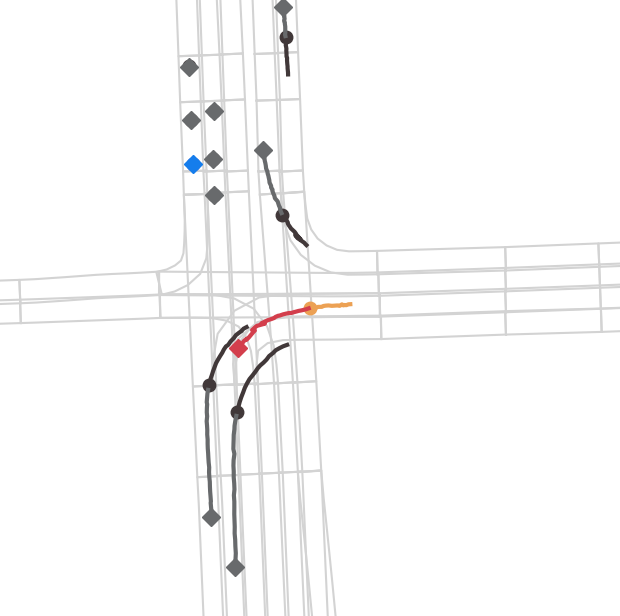
\includegraphics[width=0.23\linewidth]{5_qualitative_results_argoverse_1/val-120-general-view.png}} & 
		\fbox{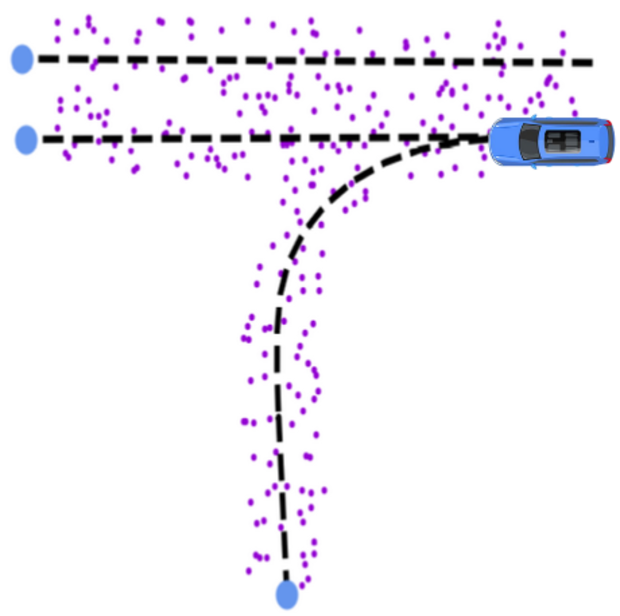
\includegraphics[width=0.23\linewidth]{5_qualitative_results_argoverse_1/val-120-plausible_hdmap.png}} &
		\fbox{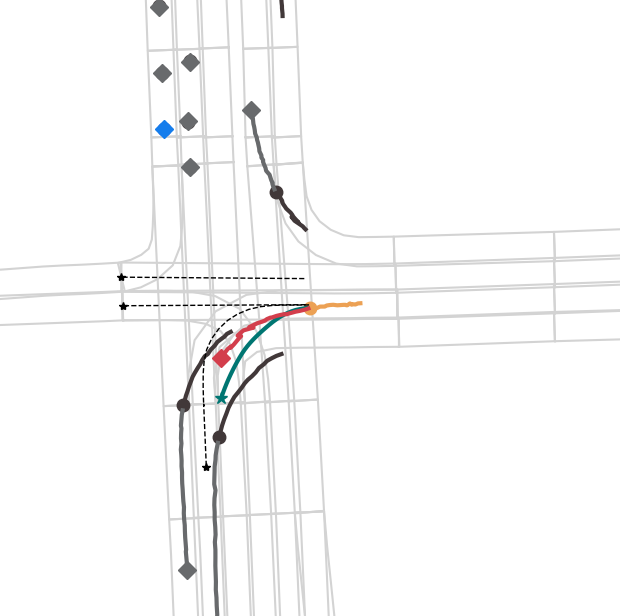
\includegraphics[width=0.23\linewidth]{5_qualitative_results_argoverse_1/val-120-unimodal.png}} & 
		\fbox{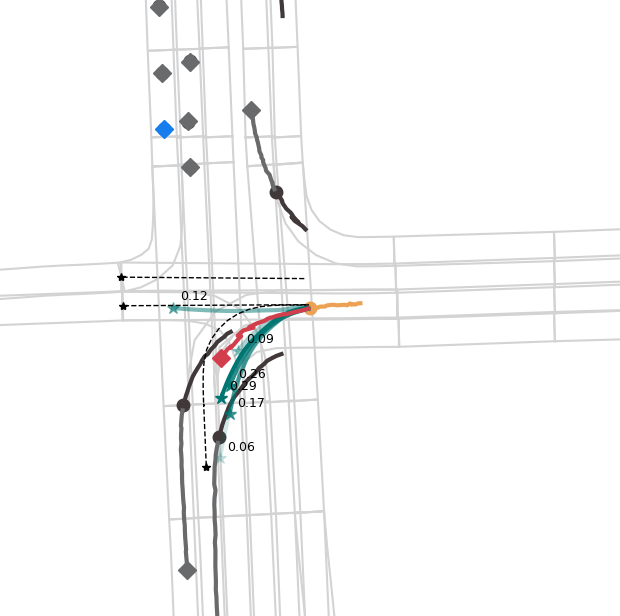
\includegraphics[width=0.23\linewidth]{5_qualitative_results_argoverse_1/val-120-multimodal_k_6.png}}
		
		\tabularnewline
		
		\fbox{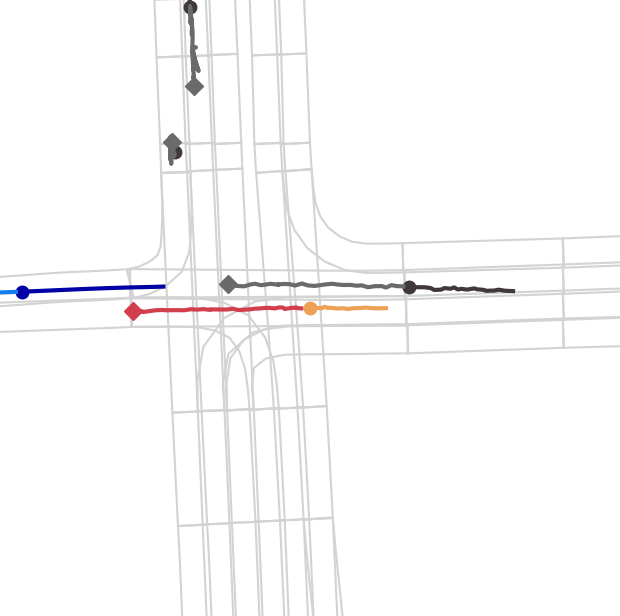
\includegraphics[width=0.23\linewidth]{5_qualitative_results_argoverse_1/val-215-general-view.png}} & 
		\fbox{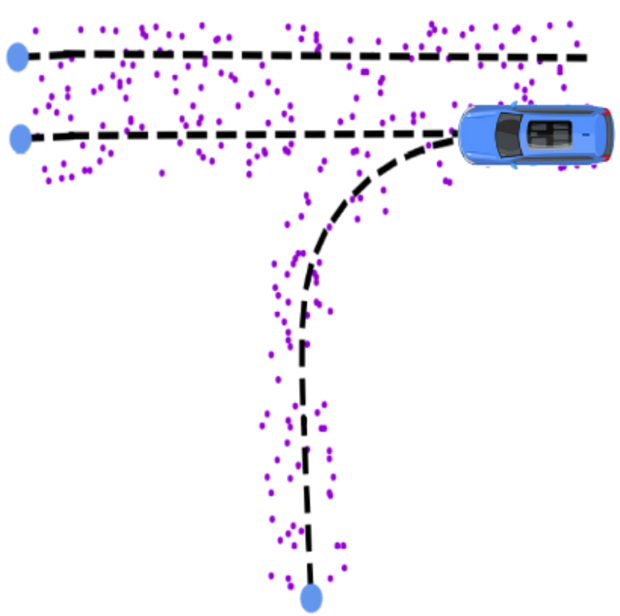
\includegraphics[width=0.23\linewidth]{5_qualitative_results_argoverse_1/val-215-plausible_hdmap.png}} &
		\fbox{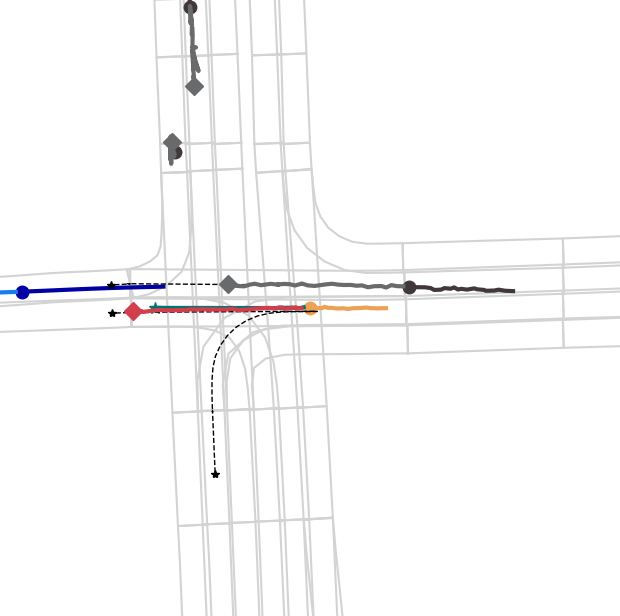
\includegraphics[width=0.23\linewidth]{5_qualitative_results_argoverse_1/val-215-unimodal.png}} & 
		\fbox{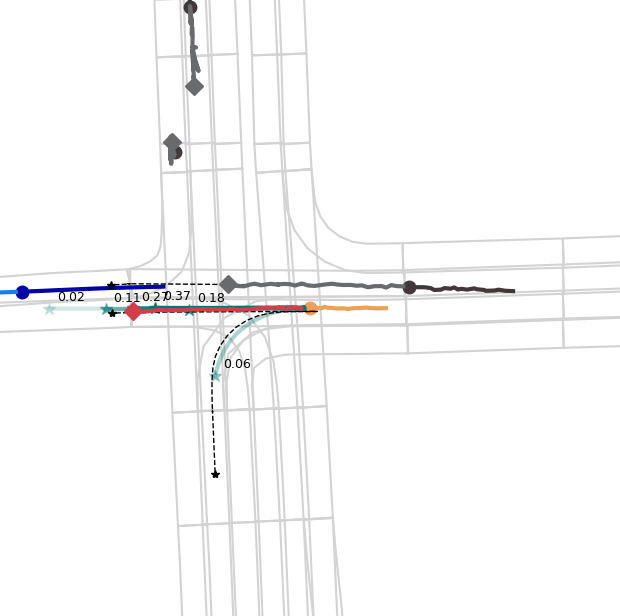
\includegraphics[width=0.23\linewidth]{5_qualitative_results_argoverse_1/val-215-multimodal_k_6.png}}
		
		\tabularnewline
		
		\fbox{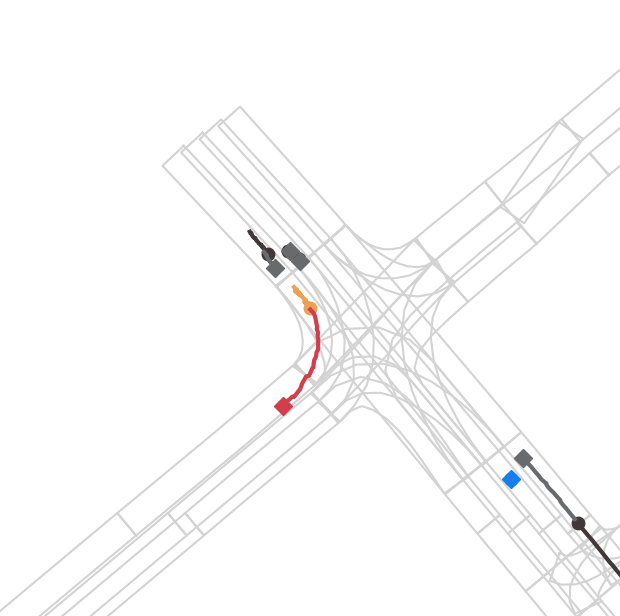
\includegraphics[width=0.23\linewidth]{5_qualitative_results_argoverse_1/val-205-general-view.png}} & 
		\fbox{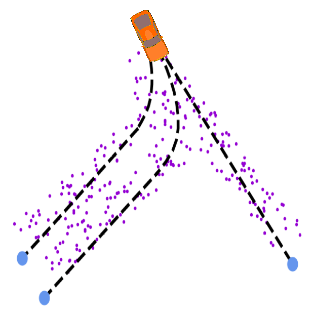
\includegraphics[width=0.23\linewidth]{5_qualitative_results_argoverse_1/val-205-plausible_hdmap.png}} &
		\fbox{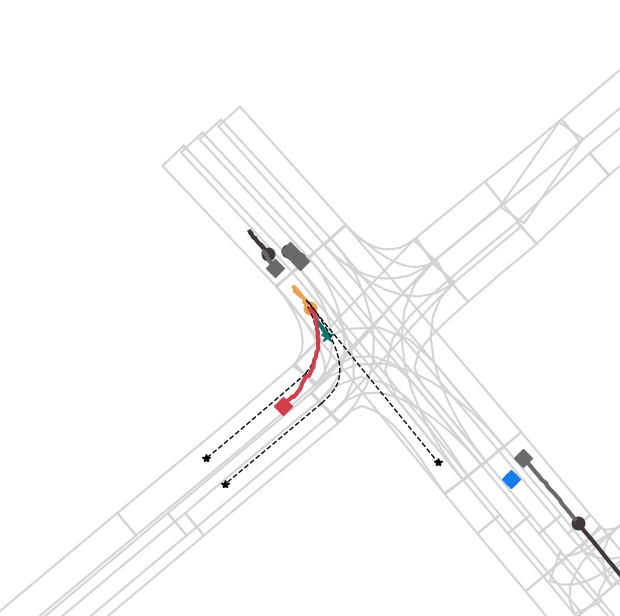
\includegraphics[width=0.23\linewidth]{5_qualitative_results_argoverse_1/val-205-unimodal.png}} & 
		\fbox{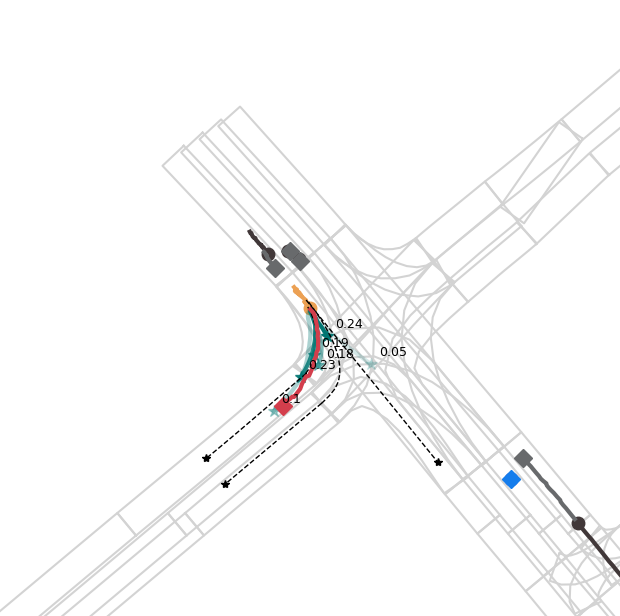
\includegraphics[width=0.23\linewidth]{5_qualitative_results_argoverse_1/val-205-multimodal_k_6.png}}
		
		\tabularnewline
		
		\fbox{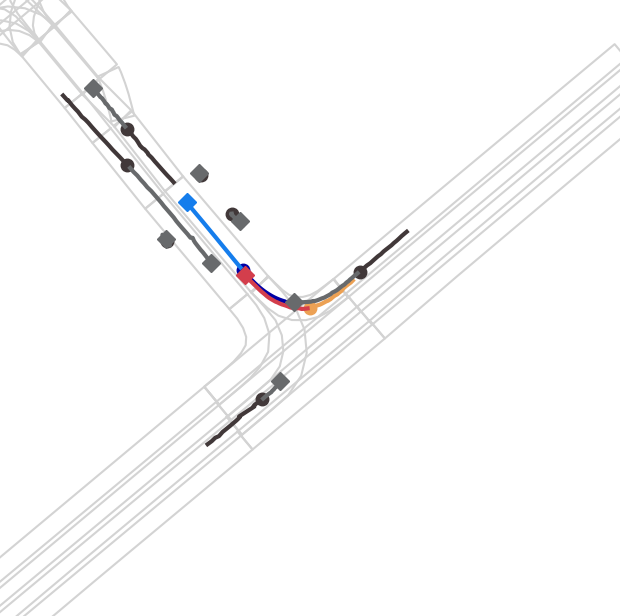
\includegraphics[width=0.23\linewidth]{5_qualitative_results_argoverse_1/val-152-general-view.png}} & 
		\fbox{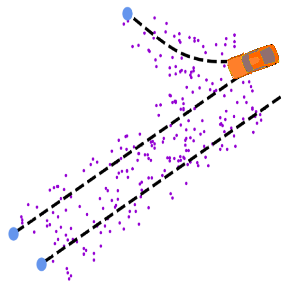
\includegraphics[width=0.23\linewidth]{5_qualitative_results_argoverse_1/val-152-plausible_hdmap.png}} &
		\fbox{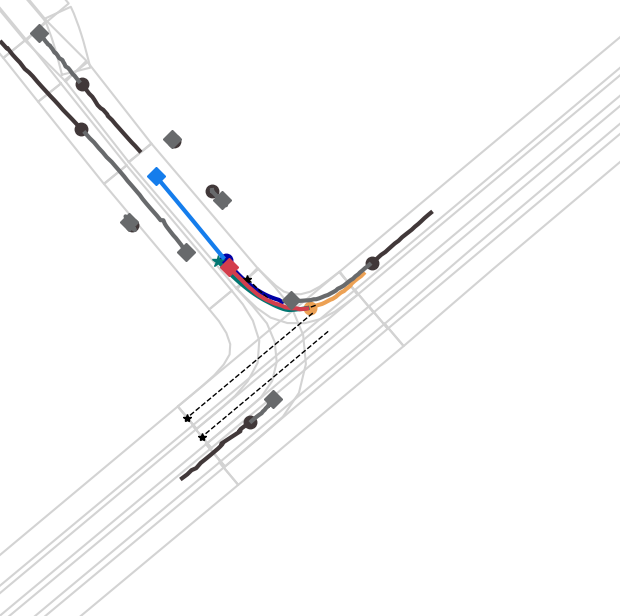
\includegraphics[width=0.23\linewidth]{5_qualitative_results_argoverse_1/val-152-unimodal.png}} & 
		\fbox{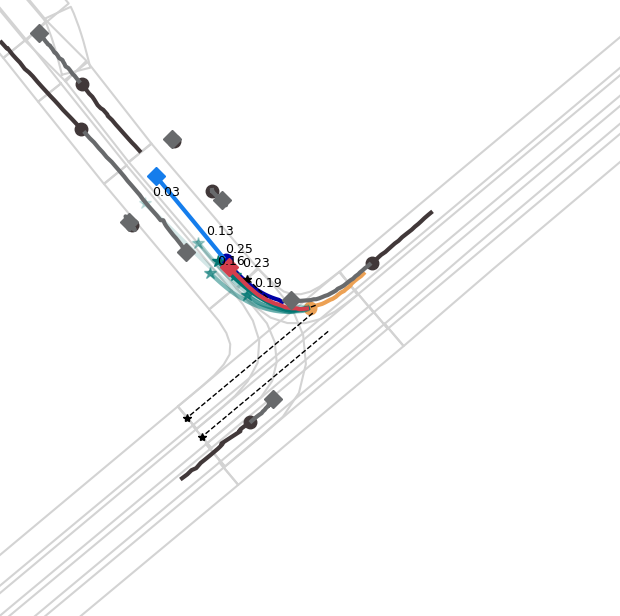
\includegraphics[width=0.23\linewidth]{5_qualitative_results_argoverse_1/val-152-multimodal_k_6.png}}
		
		\tabularnewline
		
		\fbox{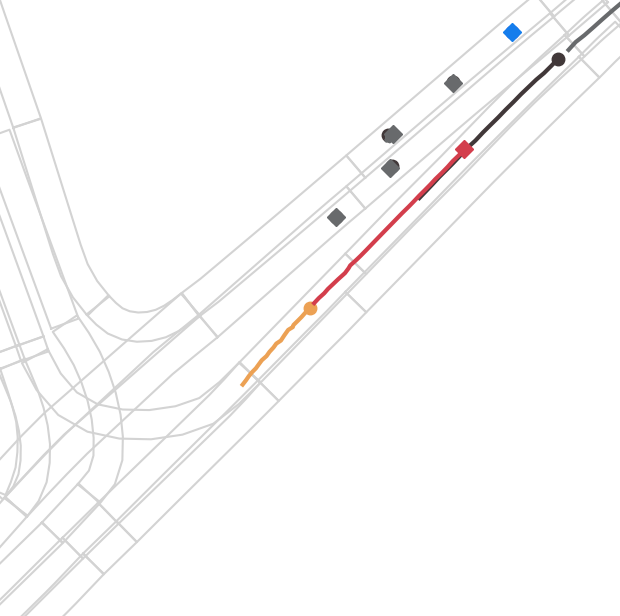
\includegraphics[width=0.23\linewidth]{5_qualitative_results_argoverse_1/val-209-general-view.png}} & 
		\fbox{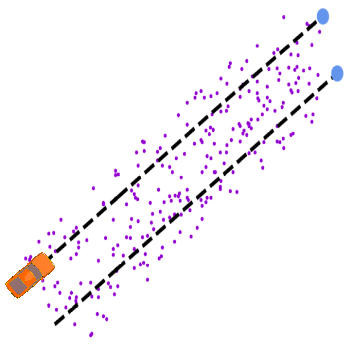
\includegraphics[width=0.23\linewidth]{5_qualitative_results_argoverse_1/val-209-plausible_hdmap.png}} &
		\fbox{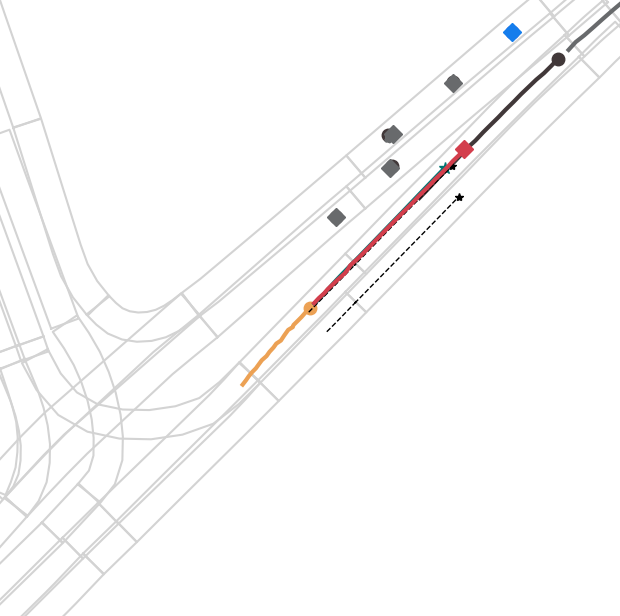
\includegraphics[width=0.23\linewidth]{5_qualitative_results_argoverse_1/val-209-unimodal.png}} & 
		\fbox{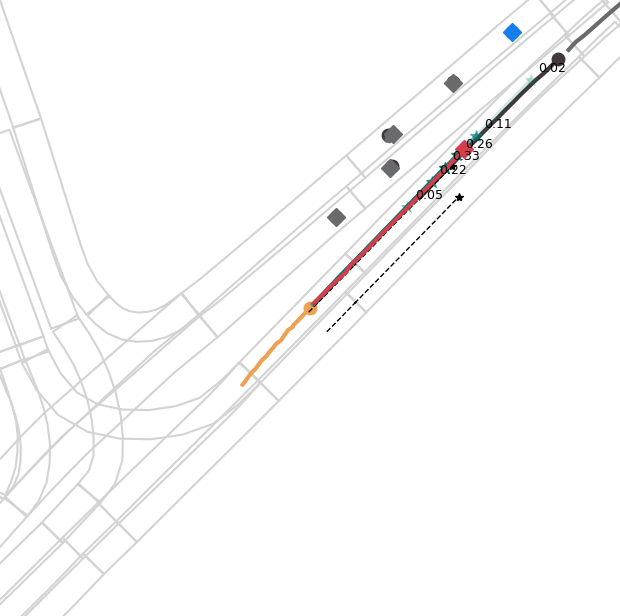
\includegraphics[width=0.23\linewidth]{5_qualitative_results_argoverse_1/val-209-multimodal_k_6.png}}
		
		\tabularnewline
		
		General view & Plausible HDMap & Unimodal (k=1) prediction & Multimodal (k=6) predictions \tabularnewline
	\end{tabular}
	\caption{Qualitative Results on challenging scenarios using our best model. %We follow the same legend and notation as in the Teaser Fig.~\ref{fig:results_teaser}.
		We represent: our vehicle (\textbf{\textcolor{blue}{ego}}), the \textbf{\textcolor{YellowOrange}{target agent}}, and \textbf{\textcolor{gray75}{other agents}}. We can also see the \textbf{\textcolor{red}{ground-truth}} trajectory of the target agent, our \textbf{\textcolor{ForestGreen}{multimodal predictions}} (with the corresponding confidences) and \textbf{plausible centerlines}. Circles represent last observations and diamonds last future positions.
		As we can see the plausible HDMap serves as a good guidance to our model, which can predict reasonable trajectories in presence of multiple agents and challenging scenarios. We show, from left to right, a general view of the traffic scenario (including social and map information), our calculated plausible HDMap, unimodal prediction (best mode in terms of confidence) and multimodal prediction (\textit{k} = 6), including confidences (the higher, the most probable)}
	\label{fig:results}
\end{figure*}

\subsection{Argoverse 2 Motion Forecasting dataset}
\label{subsec:5_argoverse_2}

Motion forecasting addresses the problem of predicting future states (or occupancy maps) for dynamic actors within a local environment.  Some examples of relevant actors for autonomous driving include: vehicles (both parked and moving), pedestrians, cyclists, scooters, and pets.  Predicted futures generated by a forecasting system are consumed as the primary inputs in motion planning, which conditions trajectory selection on such forecasts. Generating these forecasts presents a complex, multi-modal problem involving many diverse, partially-observed, and socially interacting agents. However, by taking advantage of the ability to ``self-label'' data using observed ground truth futures, motion forecasting becomes an ideal domain for application of machine learning. 

Building upon the success of Argoverse 1, the Argoverse 2 Motion Forecasting dataset provides an updated set of prediction scenarios collected from a self-driving fleet. The design decisions enumerated below capture the collective lessons learned from both our internal research/development, as well as feedback from more than 2,700 submissions by nearly 260 unique teams\footnote{This count includes private submissions not posted to the public leaderboards.} across 3 competitions \cite{argoverse_forecasting_challenge}:

\begin{itemize}
	\item \textbf{Motion forecasting is a safety critical system in a long-tailed domain.}  Consequently, our dataset is biased towards diverse and interesting scenarios containing different types of focal agents (see section \ref{mining}).  Our goal is to encourage the development of methods that ensure safety during tail events, rather than to optimize the expected performance on ``easy miles''.
	\item \textbf{There is a ''Goldilocks zone'' of task difficulty.}  Performance on the Argoverse 1 test set has begun to plateau, as shown in Figure \ref{fig:mf_score_plateau} of the appendix.  Argoverse 2 is designed to increase prediction difficulty incrementally, spurring productive focused research for the next few years.  These changes are intended to incentivize methods that perform well on extended forecast horizons (3 s $\rightarrow$ 6 s), handle multiple types of dynamic objects (1 $\rightarrow$ 5), and ensure safety in scenarios from the long tail.  Future Argoverse releases could continue to increase the problem difficulty by reducing observation windows and increasing forecasting horizons.
	\item \textbf{Usability matters.} Argoverse 1 benefited from a large and active research community---in large part due to the simplicity of setup and usage.  Consequently, we took care to ensure that existing Argoverse models can be easily ported to run on Argoverse 2.  In particular, we have prioritized intuitive access to map elements,  encouraging methods which use the lane graph as a strong prior. To improve training and generalization, all poses have also been interpolated and resampled at exactly \SI{10}{\hertz} (Argoverse 1 was approximate). The new dataset includes fewer, but longer and more complex scenarios; this ensures that total dataset size remains large enough to train complex models but small enough to be readily accessible.
\end{itemize}

\begin{table*}[!ht]
	\centering
	\caption{Comparison of methods in the \textbf{Argoverse 2 Validation} Set. We show the number of parameters for each model, prediction metrics (minADE, minFDE and brier-minFDE) for the multimodal scenario (k=6) and runtime. Runtime was measured on a single GPU A100-SXM4 (using batch 128). Our experiments are indicated using $\dagger$. We use as baseline method GANet~\cite{wang2022ganet}.}
	\resizebox{\linewidth}{!}{
		\begin{tabular}{lcccccc}
			\toprule
			Method & Map & \# Par.~(M) & minADE~(m) $\downarrow$ & minFDE~(m) $\downarrow$ & brier-minFDE~(m) $\downarrow$ & Runtime~(ms) $\downarrow$ \\
			\midrule
			GANet~\cite{wang2022ganet}                & Yes & 6.2 & 0.806 & 1.402 & 2.02 & 1612 \\
			GANet w/o Map Decoder~\cite{wang2022ganet} & Yes & 5.7 & 0.84 & 1.55 & 2.18 & 1353 \\
			GANet w/o Goal Areas~\cite{wang2022ganet} & Yes & 4.5 & 0.87 & 1.66 & 2.29 & 1134 \\
			GANet w/o map~\cite{wang2022ganet}        & No & 1.79 & 1.034 & 2.212 & 2.825 & 838 \\
			%social only
			$\dagger$ CRAT-Pred~\cite{schmidt2022crat} & No & 0.53 & 1.31 & 2.78 & 3.65 & 223 \\
			\midrule
			$\dagger$ Ours-base: GANet~\cite{wang2022ganet} ~~~ActorNet $\rightarrow$ Attention Transformer & Yes & 5.0 & 0.83 & 1.45 & 2.07 & 923 \\
			$\dagger$ Ours-m: Ours-base + A2A $\rightarrow$ C-GCN + Metadata  & Yes & 4.74 & 0.82 & 1.43 & 2.05 & 892 \\
			% Ours-s = dim=64 --> smaller version
			$\dagger$ Ours-s: Ours-base + A2A $\rightarrow$ C-GCN + Metadata (64 latent size) & Yes & 1.2 & 0.88 & 1.53 & 2.15 & 893 \\
			% Ours final
			$\dagger$ \textbf{Ours:} Ours-m + Proposals + Motion Refinement & Yes & 4.92 & 0.81 & 1.42 & 2.04 & 946 \\
			\bottomrule
		\end{tabular}
	}
	\label{table:table_1}
\end{table*}

\begin{table*}[!ht]
	\small
	\caption{Results on \textbf{Argoverse 2 Test} dataset. The "-" denotes that this result was not reported in their paper. Some numbers are borrowed from~\cite{wang2022ganet}. For all the metrics, the lower, the better.}
	\label{test}
	\centering
	\resizebox{\linewidth}{!}{
	\begin{tabular}{cccccccc}
		\toprule
		Method     &\makecell[c]{b-minFDE\\(K=6)} &\makecell[c]{MR\\(K=6)} &\makecell[c]{minFDE\\(K=6)} &\makecell[c]{minADE\\(K=6)} &\makecell[c]{minFDE\\(K=1)} &\makecell[c]{minADE\\(K=1)} &\makecell[c]{MR\\(K=1)} \\
		\midrule
		
		DirEC &3.29  &0.52 &2.83 &1.26 &	6.82 &	2.67 &0.73    \\
		
		drivingfree&3.03 &	0.49 &2.58 &1.17 &6.26 & 2.47 &0.72     \\
		
		LGU	&2.77 & 0.37 & 2.15 &1.05 &6.91 & 2.77 & 0.73 \\
		
		Autowise.AI(GNA) &2.45	&0.29 &1.82	&0.91 &6.27	& 2.47  &	0.71\\
		
		Timeformer~\cite{gilles2021thomas}   &2.16	&0.20 &1.51 & 0.88 &4.71	&1.95 &0.64\\
		
		QCNet    &2.14	&0.24 &1.58 &0.76	&4.79 & 1.89 &0.63 \\
		
		\textit{OPPred w/o Ensemble}~\cite{zhang2022banet} 	&2.03	&0.180 & 1.389		&0.733	&4.70	&1.84  &0.615\\
		
		\textit{TENET w/o Ensemble}~\cite{wang2022tenet}&2.01&- &-	&-	&-	&-&-\\
		
		Polkach(VILaneIter)  &2.00	&0.19 & 1.39	&\textbf{0.71}	&4.74	&1.82	&0.61 \\
		
		GANet &\textbf{1.969}	& \textbf{0.171} &\textbf{1.352}	&0.728 &\textbf{4.475} &\textbf{1.775} &\textbf{0.597}	 \\
		
		\midrule
		Ours & 1.98 & 0.185 & 1.37 & 0.73 & 4.53 & 1.79 & 0.608 \\
		\bottomrule
	\end{tabular}}
	\label{table:table_2}
\end{table*}

% of 0.0001. 

% Where $\alpha=1.0$ , $\beta=0.1$ and $\gamma=0.65$ initially, and can be manually adjusted during training (especially $\gamma$).

\subsection{Implementation Details}

We train our models to convergence using a single NVIDIA \textbf{RTX 3090}, and validate our results on the official Argoverse validation set~\cite{chang2019argoverse}. We use Adam optimizer with learning rate $0.001$ and default parameters, batch size $1024$ and linear LR Scheduler with factor $0.5$ decay on plateaus. We rotate the whole scene regarding the orientation in the last observation frame of the target agent to align this agent with the positive y-axis. The hidden dimension for the Motion History encoder is 64, where both the hidden state $\mathbf{h_{in}}$ and cell state $\mathbf{c_{in}}$ are initialized with zeros (dim = $128$), whilst the MLP encoder for both the specific centerline and plausible area is 128. Regarding the Social Interaction module, the latent vector of the Crystal-GCN layers is 128 and the number of heads in the MHSA module is $L_h = 4$. In terms of the Autoregressive predictor, the spatial embedding and \textit{dist2centerline} modules encode the past data and distance to the specific centerline using a \textit{window size} of 20. We set the number of plausible centerlines (\textit{M}) as 3, which cover most cases (if less than 3 plausible centerlines are available, we add padded centerlines as vector of zeros). The time tensor is a single number that represents the current timestep, in such a way the LSTM input is \textit{(2 $\times$ window size) + 1 = 41}. The regression head is represented by \textit{k=6} FC layers that map the output latent vector returned by the LSTM to the final output relative displacements (dim = 2, xy). Multimodal predictions are processed by an MLP residual of sizes 60, 60 and 6 with interspersed ReLU activations in order to obtain the corresponding confidences.

\paragraph{Augmentations} 

(i) Dropout and swapping random points from the past trajectory, (ii) point location perturbations under a $\mathcal{N}(0, 0.2)$ [m] noise distribution~\cite{ye2021tpcn}. We also apply the well-known hard-mining technique to improve the model's generalization under difficult scenarios. To perform this technique, once we have the social and map baselines, we perform inference on the training set to find the most difficult scenes in terms of minADE. Then, we mine those scenes such that the baselines models perform poorly, and increase their proportion in the batch during training.

% Additional bio: dong2017hardmine

\section{Decision-Making}

The increasing popularity of autonomous vehicles (AVs) has brought with it significant challenges in ensuring safe and effective decision-making, particularly in complex urban driving scenarios \cite{Yurtsever2019}. Reinforcement learning (RL) techniques have emerged as a promising solution to address these challenges \cite{Ravi2020}. They enable AVs to learn from their interactions with the driving environment, without relying on pre-defined rules. However, RL-based approaches still face a number of limitations that can hinder their development, including issues related to state representation.

A key challenge in RL-based AVs is the development of effective state representations that can account for the complexity of urban driving scenarios. Unlike in simpler environments, state representations for urban driving must be able to incorporate a wide range of information, including dynamic features of traffic flows and interactions among different agents. Finding ways to effectively encode this information and develop accurate state representations is essential to enabling RL-based AVs to generalize to various scenarios and make effective driving decisions. Distilling predictive information from scene representations can aid in the development of effective decision-making policies for AVs. By better understanding the potential consequences of different driving actions, RL-based AVs can make more informed decisions that lead to safer and more efficient driving behaviour.

This paper proposes an approach to enhance the efficiency and generalization of RL-based AVs in urban driving scenarios. Specifically, we introduce the use of a Motion Prediction (MP) module to obtain the future positions of the vehicles in the scenario. These predictions are the input to an RL-based decision-making module that executes high-level actions. Our approach is developed using the Proximal Policy Optimization (PPO) algorithm  \cite{Schulman2017}.  We carry out an evaluation in the unsignalized T-intersection scenario shown in Fig. \ref{fig:teaser} with and without the proposed state representation and provide a comparison with some baseline methods.

\begin{figure*}[ht]
	\centering
	\begin{subfigure}{0.4\textwidth}
		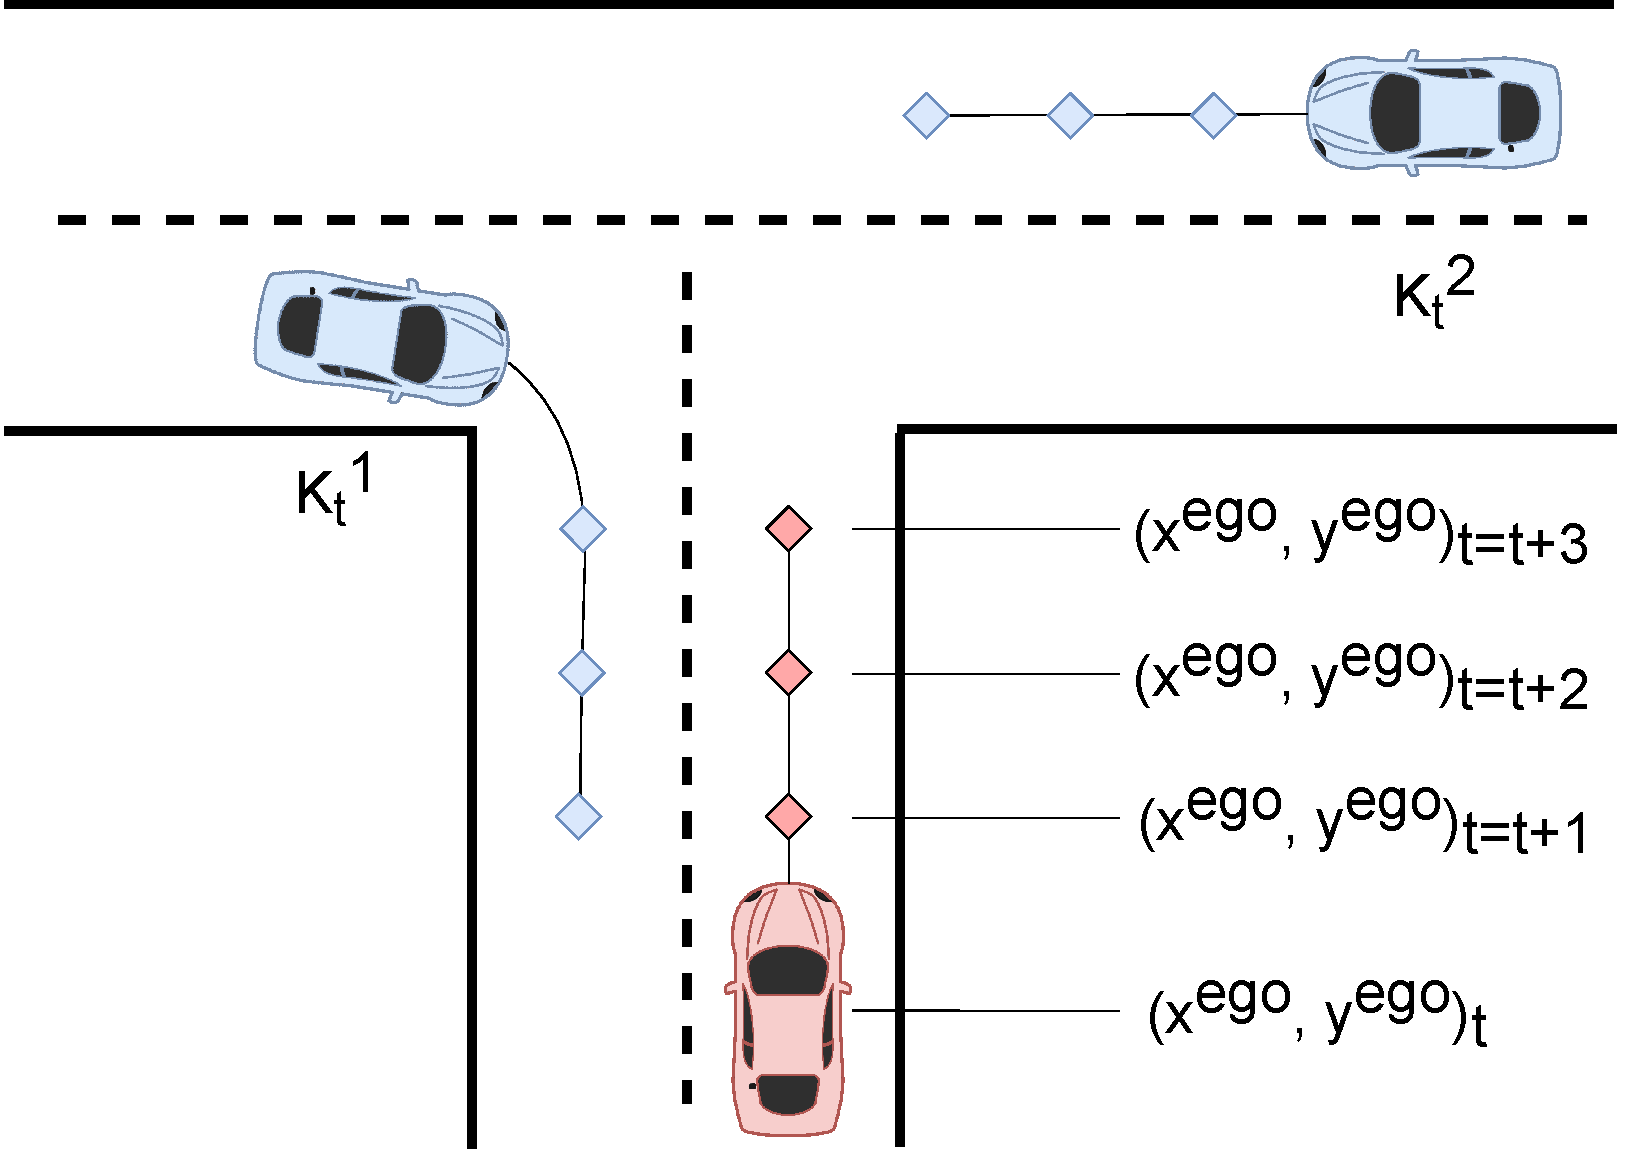
\includegraphics[width=\textwidth]{5_dm_state}
		\caption{Space state}
	\end{subfigure}
	\hfill
	\begin{subfigure}{0.5\textwidth}
		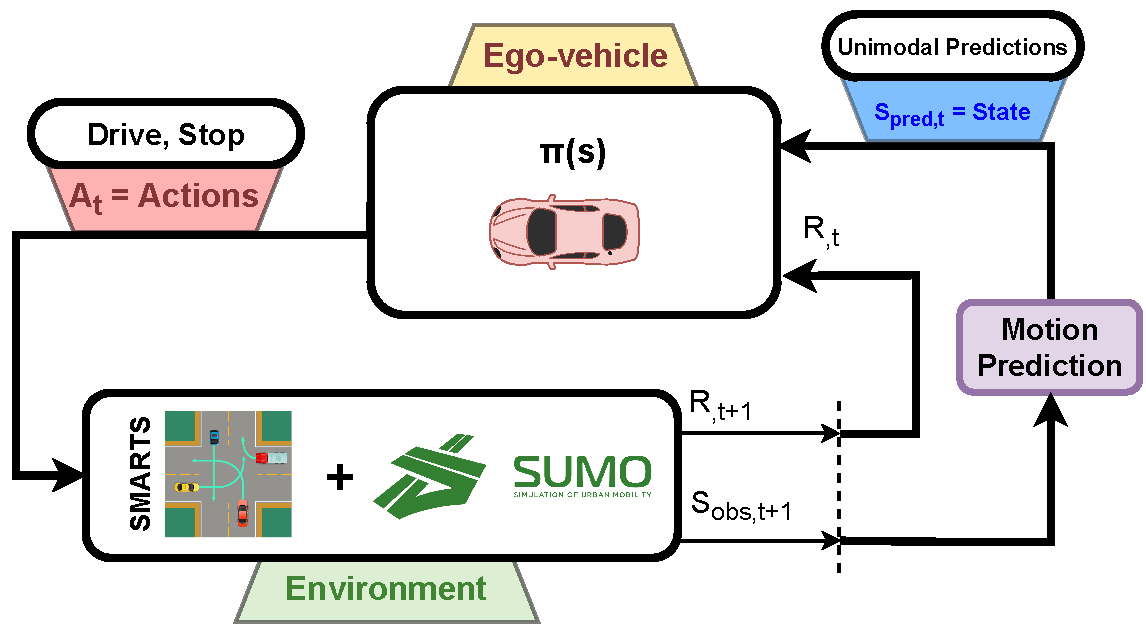
\includegraphics[width=\textwidth]{5_dm_pipeline.pdf}
		\caption{Autonomous Decision Making based on Reinforcement Learning using Unimodal Predictions as input}
	\end{subfigure}
	
	\label{fig:5_decision_making}
\end{figure*}

\label{sec:5_decision_making}

% https://xindiwu.github.io/data/motion.pdf

\section{Holistic Simulation in CARLA}

\label{sec:5_simulation}

\section{Summary}
\label{sec:5_summary}